\chapter{Writing a Source-to-Source Translator}

\label{translatorDesign:translatorDesign}

% Purpose:
%\begin{itemize}
%   \item A. Section overview
%   \item B. Why you should read this manual
%   \item C. How to use this manual
%   \item D. Terminology
%   \item E. Overview of library
%   \item F. Program control
%   \item G. Error messages
%   \item H. Section summary
%\end{itemize}

\section{Introduction}

   All source-to-source translators (also referred to as translators within some parts of
this documentation) can be expected to share a common simple design for their {\tt main()}
function.  Translators can be expected to be implemented by calling different
functions operating on the AST (either reading or reading and writing to the AST).
This chapter presents the common design of the {\tt main()} for all translators
built using ROSE.  The user's {\tt main()} function will amount to a few lines 
of code only, but it will set the framework within which we can explain how to use 
other mechanisms within ROSE to build more interesting (complex) translators.

\section{Example Translator}

   This section shows a simple translator and a trivial modification to it
to permit the AST to be dumped out as a clickable PDF file. The purpose
of this section is only to show an example translator. The added modification is
only included to make the example a little more interesting.

   Nearly all translators can be expected to have a similar design, but include a
separate function call to process the AST. The other chapters in this ROSE manual
depend upon a simple understanding of this section.  Other chapters, in particular
the AstProcessing and AstRewrite chapters will detail how to build alternative
functions which will read or read/write the AST.  The AST is the principal
data structure which is modified to introduce transformations in any input application.

\subsection{A Simple Translator}

   The example code \ref{translatorDesign:simpleTranslator} shows a complete
code representing a simple example translator which will:
\begin{enumerate}
     \item Accept an input application code (written in C or C++)
     \item Internally process the application code
     \begin{enumerate}
          \item Parse the input application code
          \item Generate an AST representing the input application code
     \end{enumerate}
     \item generate a new file semantically identical to the input file
     \item compile the generated code using the back-end C++ compiler
\end{enumerate}

{\indent
{\mySmallFontSize

% Do this when processing latex to generate non-html (not using latex2html)
\begin{latexonly}
%  \lstinputlisting{\TranslatorExampleDirectory/identityTranslator.C}
\begin{figure}[tb]
\begin{center}
\begin{tabular}{|c|} \hline
     Simple Source-to-Source Translator
\\\hline\hline
\lstinputlisting{\TranslatorExampleDirectory/identityTranslator.C}
\\\hline
\end{tabular}
\end{center}
\caption{ Example of simple translator, building and AST, unparsing it, and compiling
    the generated (unparsed) code. }
\end{figure}
\end{latexonly}

% Do this when processing latex to build html (using latex2html)
\begin{htmlonly}
   \verbatiminput{\TranslatorExampleDirectory/identityTranslator.C}
\end{htmlonly}

\label{translatorDesign:simpleTranslator}

%end of scope in font size
}
% End of scope in indentation
}

   This simple example translator is admittedly not particularly useful since it effectively
only calls the C++ compiler through a level of indirection (parsing and regenerating
the original application unchanged).  The next section shows a simple modification of this
translator to dump out the AST as a PDF file.

\fixme{Fixme Note: Should we add the modification required to output a Dot file representing the AST?}

\subsection{Modifying the Simple Translator to output the AST}

   We can easily modify this simple example translator to do something a little more
interesting; visualizing the internal AST (not possible with a typical vendor's compiler).
To do this we add a few extra lines shown in \ref{translatorDesign:outputAstCodeFragment}.

{\indent
{\mySmallFontSize

% Do this when processing latex to generate non-html (not using latex2html)
\begin{latexonly}
%  \lstinputlisting{\TranslatorExampleDirectory/identityTranslator.C}
\begin{figure}[tb]
\begin{center}
\begin{tabular}{|c|} \hline
     Additional lines required to output AST
\\\hline\hline
\lstinputlisting{\TranslatorExampleDirectory/astOutput.codeFragment}
\\\hline
\end{tabular}
\end{center}
\caption{ Code fragment required to output AST as a PDF file (suitable for larger input files). }
\end{figure}
\end{latexonly}

% Do this when processing latex to build html (using latex2html)
\begin{htmlonly}
   \verbatiminput{\TranslatorExampleDirectory/astOutput.codeFragment}
\end{htmlonly}

\label{translatorDesign:outputAstCodeFragment}

%end of scope in font size
}
% End of scope in indentation
}

Putting this code fragment into the previous simple example translator we build
a translator that can dump out the internal AST (we skip the unparsing of the AST and
the compilation of the generated code). The resulting code is shown in 
\ref{translatorDesign:AstPDFOutputTranslator}.
The result of this translator is a PDF representation of the AST representing any
input application.  This feature is particularly useful for debugging transformations 
and translators that perform analysis.

{\indent
{\mySmallFontSize

% Do this when processing latex to generate non-html (not using latex2html)
\begin{latexonly}
%  \lstinputlisting{\AstRewriteExampleDirectory/identityTranslator.C}
\begin{figure}[tb]
\begin{center}
\begin{tabular}{|c|} \hline
     Simple Source-to-Source Translator
\\\hline\hline
\lstinputlisting{\TranslatorExampleDirectory/AstPdfOutputTranslator.C}
\\\hline
\end{tabular}
\end{center}
\caption{ Example of simple translator, building and AST, unparsing it, and compiling
    the generated (unparsed) code. }
\end{figure}
\end{latexonly}

% Do this when processing latex to build html (using latex2html)
\begin{htmlonly}
   \verbatiminput{\TranslatorExampleDirectory/AstPdfOutputTranslator.C}
\end{htmlonly}

\label{translatorDesign:AstPDFOutputTranslator}

%end of scope in font size
}
% End of scope in indentation
}

% \fixme{We need a picture of the PDF version of the documentation.}

The output of this translator is shown in figure \ref{}.  The left hand side
of the screen is a tree with click-able nodes to expand/collapse the subtrees.
The right hand side of the screen is a description of the data at a particular 
node in the AST (the node where the user has clicked the left mouse button).
This relatively simple view of the AST is useful for debugging transformation and finding
information in the AST required by specific sorts of analysis.  It is also useful
for developing an intuitive feel for what information is in the AST, how it is organized, 
and where it is stored.

\begin{figure}
\centerline{\epsfig{file=\TranslatorExampleDirectory/AST-pdf2.ps,height=0.75\linewidth,width=1.0\linewidth,angle=0}}
\caption{Example output from translator which outputs PDF representation of AST.}
\label{translatorDesign:pdfOutput1.ps}
\end{figure}

    A similar (alternative) representation is possible which provides a graph 
representation \ref{translatorDesign:dotOutput1.ps}.

\begin{figure}
\centerline{\epsfig{file=\TranslatorExampleDirectory/AST-dot1.ps,height=0.75\linewidth,width=1.0\linewidth,angle=0}}
\caption{Example output from translator which outputs DOT (graph) representation of AST.}
\label{translatorDesign:dotOutput1.ps}
\end{figure}

\section{Translator with AST Traversal}

   This section forms an example that will be used is subsequent chapters.
Specifically it shows the code required for a translator that will
traverse the AST.  In subsequent chapters only the traversal object will be
exchanged to build translators with greater complexity.
In the example translator \label{translatorDesign:AstTraversalTranslator}
an {\tt AstSimpleProcessing} object is constructed and called. The AST Processing
chapter \ref{AstProcessing:AstProcessing} will detail the different forms of
AST processing that are available within ROSE.

{\indent
{\mySmallFontSize

% Do this when processing latex to generate non-html (not using latex2html)
\begin{latexonly}
%  \lstinputlisting{\AstRewriteExampleDirectory/identityTranslator.C}
\begin{figure}[tb]
\begin{center}
\begin{tabular}{|c|} \hline
     Simple Source-to-Source Translator
\\\hline\hline
\lstinputlisting{\TranslatorExampleDirectory/AstTraversalTranslator.C}
\\\hline
\end{tabular}
\end{center}
\caption{ Example of simple translator, building and AST, unparsing it, and compiling
    the generated (unparsed) code. }
\end{figure}
\end{latexonly}

% Do this when processing latex to build html (using latex2html)
\begin{htmlonly}
   \verbatiminput{\TranslatorExampleDirectory/AstTraversalTranslator.C}
\end{htmlonly}

\label{translatorDesign:AstTraversalTranslator}

%end of scope in font size
}
% End of scope in indentation
}

Because we present this example here, subsequent chapters can restrict themselves to
the presentation of examples showing the design of the traversal and reference this
example code for the complete translator definition.

\section{Adding Command Line Processing}

   ROSE passes all non-ROSE and non-EDG specific command line options to the backend
compiler.  This simple model assures that any translator built using ROSE can be used
in place of the vendors compiler. ROSE includes command line processing that is 
specific to ROSE as well as some limited command line processing specific to EDG
(EDG specific command line options will be expanded at some point).

   The user can use the same mechanism that we use internally in ROSE to handle command
line processing.  Specifically we use the SLA command line processing, built by Brian 
Gunney (now at LLNL).  Specific documentation for SLA is available, likely from Brian 
directly or from the ROSE team, but it is simple enough that we hope that a few comments and
an example will be sufficient.

   The example below shows the command line processing associated with a simple
help option.  Either {\tt --h} or {\tt --help} are sufficient as command line options.
The first two options are {\tt argc} and {\tt argv}; standard inputs to 
{\tt main(int argc, char* argv[])}.  The third option is the prefix string to the option.
The fourth parameter is the something; I don't remember :-).
The fifth parameter is the suffix string to the option parameter.
The final option is either 1 or 0: 1 removes the option from the command line and 0 leaves
the option in place within the command line.

The second example use of SLA in the example code shows how to configure a option that
takes a parameter. It is hopefully self explanatory.

{\indent
{\mySmallFontSize

% Do this when processing latex to generate non-html (not using latex2html)
\begin{latexonly}
\begin{figure}[tb]
\begin{center}
\begin{tabular}{|c|} \hline
     Simple Command Line Processing Example Translator
\\\hline\hline
\lstinputlisting{\TranslatorExampleDirectory/commandLineProcessingExample.C}
\\\hline
\end{tabular}
\end{center}
\caption{ Example of simple command line processing using SLA library. }
\end{figure}
\end{latexonly}

% Do this when processing latex to build html (using latex2html)
\begin{htmlonly}
   \verbatiminput{\TranslatorExampleDirectory/commandLineProcessingExample.C}
\end{htmlonly}

\label{translatorDesign:commandLineProcessing}
}
}

\section{Commandline Processing}

   Translators built using ROSE contain some default command-line options that
are specific general processing.  The user building his own translator may add 
their own command line options using same mechanism used internally in ROSE.
ROSE uses a command-line processing package,String List Assignment (SLA), written 
by Brian Gunney (at LLNL).  The complete distribution of SLA is included in the
CVS repository for developers, and could later be included in the ROSE distribution.
Complete documentation is contained in the SLA distribution.  


\section{Conclusions}

   The development of a translator using ROSE is particularly simple.  The point
of this chapter has been to introduce the basics of how abstractions in ROSE make this
simple for users.  Clearly, at this point in the presentation of ROSE, no compiler 
background is required to build such translators.  Importantly, most translators 
involve a {\tt main()} function which is not much more complex that the ones presented
in this chapter.





